
Let the given points 

\begin{align}
    \vec{A}=\myvec{h\\3}
    \\
    \vec{B}=\myvec{4\\1}
\end{align}

Directional vector of line passing through points $\vec{A}$ and $\vec{B}$ is
\begin{align}
  \vec{P} &= \vec{B}-\vec{A}
  \\
  \vec{P} &= \myvec{h-4\\2}
\end{align}
 Directional vector of the line $\myvec{ a & b }\vec{x}=c$ is 

\begin{align}
  \vec{Q} &= \myvec{b\\-a}
  \label{eq:solutions/line_plane/39/1}
\end{align}

From \eqref{eq:solutions/line_plane/39/1} direction vector of line $\myvec{7 & -9}\vec{x}=19$ is
\begin{align}
  \vec{Q} &= \myvec{-9\\-7}
\end{align}

If two straight lines intersects at right angles then inner product of their directional vectors is zero.
\begin{align}
    \vec{P}^T\vec{Q}=0
    \\
    %\vspace{5cm}
    \myvec{h-4\\2}^T\myvec{-9\\-7}=0
    \\
    \myvec{h-4 & 2}\myvec{-9\\-7}=0
    \\
    (h-4)(-9)+2(-7)=0
    \\
    h=\dfrac{22}{9} \label{eq:solutions/line_plane/39/u2}
\end{align}


Python Plot used to verify the result obtained from \eqref{eq:solutions/line_plane/39/u2}.

\begin{figure}[h!] 
	\centering
	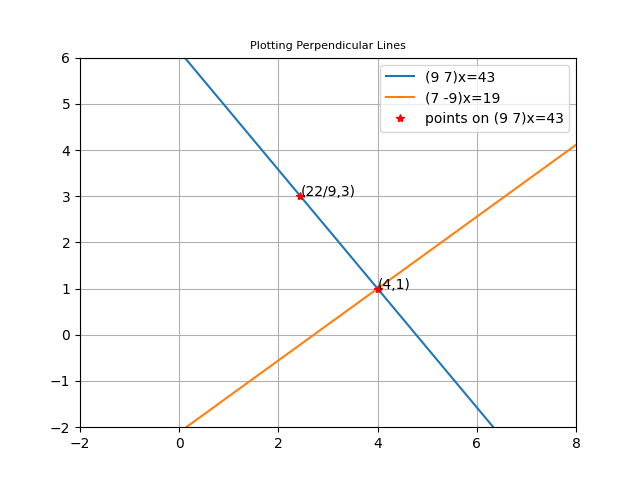
\includegraphics[width=\columnwidth]{./solutions/line_plane/39/assignment1_method2_plot.png}
	\caption{Figure showing given data and corresponding results}
	\label{myfig:solutions/line_plane/39/}
\end{figure}

According to the problem statement, equation of line passing through the point $\myvec{ 4 \\ 1 }$ and perpendicular to the line $\myvec{ 7 & -9 }\vec{x}=19$ is 
\begin{align}
  \myvec{ 9 & 7 }\vec{x}=43
  \label{eq:solutions/line_plane/39/u3}
\end{align}

Fig. \ref{myfig:solutions/line_plane/39/} shows that equation \eqref{eq:solutions/line_plane/39/u3} passes through the point $\myvec{ \dfrac{22}{9} \\ \\ 3}$

